% Options for packages loaded elsewhere
\PassOptionsToPackage{unicode}{hyperref}
\PassOptionsToPackage{hyphens}{url}
%
\documentclass[
  9pt,
  ignorenonframetext,
]{beamer}
\usepackage{pgfpages}
\setbeamertemplate{caption}[numbered]
\setbeamertemplate{caption label separator}{: }
\setbeamercolor{caption name}{fg=normal text.fg}
\beamertemplatenavigationsymbolsempty
% Prevent slide breaks in the middle of a paragraph
\widowpenalties 1 10000
\raggedbottom
\setbeamertemplate{part page}{
  \centering
  \begin{beamercolorbox}[sep=16pt,center]{part title}
    \usebeamerfont{part title}\insertpart\par
  \end{beamercolorbox}
}
\setbeamertemplate{section page}{
  \centering
  \begin{beamercolorbox}[sep=12pt,center]{part title}
    \usebeamerfont{section title}\insertsection\par
  \end{beamercolorbox}
}
\setbeamertemplate{subsection page}{
  \centering
  \begin{beamercolorbox}[sep=8pt,center]{part title}
    \usebeamerfont{subsection title}\insertsubsection\par
  \end{beamercolorbox}
}
\AtBeginPart{
  \frame{\partpage}
}
\AtBeginSection{
  \ifbibliography
  \else
    \frame{\sectionpage}
  \fi
}
\AtBeginSubsection{
  \frame{\subsectionpage}
}
\usepackage{lmodern}
\usepackage{amsmath}
\usepackage{ifxetex,ifluatex}
\ifnum 0\ifxetex 1\fi\ifluatex 1\fi=0 % if pdftex
  \usepackage[T1]{fontenc}
  \usepackage[utf8]{inputenc}
  \usepackage{textcomp} % provide euro and other symbols
  \usepackage{amssymb}
\else % if luatex or xetex
  \usepackage{unicode-math}
  \defaultfontfeatures{Scale=MatchLowercase}
  \defaultfontfeatures[\rmfamily]{Ligatures=TeX,Scale=1}
\fi
\usetheme[]{Goettingen}
\usecolortheme{rose}
% Use upquote if available, for straight quotes in verbatim environments
\IfFileExists{upquote.sty}{\usepackage{upquote}}{}
\IfFileExists{microtype.sty}{% use microtype if available
  \usepackage[]{microtype}
  \UseMicrotypeSet[protrusion]{basicmath} % disable protrusion for tt fonts
}{}
\makeatletter
\@ifundefined{KOMAClassName}{% if non-KOMA class
  \IfFileExists{parskip.sty}{%
    \usepackage{parskip}
  }{% else
    \setlength{\parindent}{0pt}
    \setlength{\parskip}{6pt plus 2pt minus 1pt}}
}{% if KOMA class
  \KOMAoptions{parskip=half}}
\makeatother
\usepackage{xcolor}
\IfFileExists{xurl.sty}{\usepackage{xurl}}{} % add URL line breaks if available
\IfFileExists{bookmark.sty}{\usepackage{bookmark}}{\usepackage{hyperref}}
\hypersetup{
  pdftitle={BIOS6643 Longitudinal},
  pdfauthor={EJC},
  hidelinks,
  pdfcreator={LaTeX via pandoc}}
\urlstyle{same} % disable monospaced font for URLs
\newif\ifbibliography
\setlength{\emergencystretch}{3em} % prevent overfull lines
\providecommand{\tightlist}{%
  \setlength{\itemsep}{0pt}\setlength{\parskip}{0pt}}
\setcounter{secnumdepth}{-\maxdimen} % remove section numbering
\AtBeginSubsection{}
\AtBeginSection{}
\ifluatex
  \usepackage{selnolig}  % disable illegal ligatures
\fi

\title{BIOS6643 Longitudinal}
\subtitle{L14 GEE}
\author{EJC}
\date{}
\institute{Department of Biostatistics \& Informatics}

\begin{document}
\frame{\titlepage}

\begin{frame}[allowframebreaks]
  \tableofcontents[hideallsubsections]
\end{frame}
\hypertarget{gee}{%
\section{GEE}\label{gee}}

\begin{frame}{Topics for today}
\protect\hypertarget{topics-for-today}{}
\begin{itemize}
\item
  When to use non-normal methods
\item
  Interpreting effects in loglinear and logistic models
\item
  Augmenting GzLMs to account for correlated responses
\item
  Related reading:

  \begin{itemize}
  \item
    Sections 1 through 4 in the Non-normal notes {[}Section 3 was
    covered in more detail by Gary Grunwald{]}
  \item
    Section 7 `Interpreting effects for loglinear and logistic models'
    in the `Interpreting parameters in longitudinal models' chapter.
  \end{itemize}
\end{itemize}
\end{frame}

\begin{frame}[fragile]{Introduction}
\protect\hypertarget{introduction}{}
\begin{verbatim}
- Topic:  models for outcome variables that are not normally distributed.

- Methods for modeling non-normal correlated data are also discussed in BIOS7712.  

- We have learned how to use linear mixed models to fit clustered data with continuous and approximately normally distributed outcome variables.  The models are versatile in handling random effects as well as repeated measures over time.  

- For other types of outcome variables that involve clustered data, such as counts or binary outcomes, we can use generalized estimating equations (GEE) or employ generalized linear mixed models (GzLMM) as discussed in this chapter.
\end{verbatim}
\end{frame}

\hypertarget{gzlmm}{%
\section{GzLMM}\label{gzlmm}}

\begin{frame}{Determining when and when not to use normal theory
methods}
\protect\hypertarget{determining-when-and-when-not-to-use-normal-theory-methods}{}
\begin{itemize}
\item
  A normal-theory model (e.g., GLM, LMM) may work adequately for a given
  outcome even if it is not perfectly normal. Typically, the model fit
  will be fairly robust to violations of the normal assumption as long
  as the distribution is not too skewed or does not have a high
  percentage of data on one or more individual values, or when sample
  sizes are large enough that the central limit theorem comes into play.
\item
  Sometimes we can still employ normal theory models even when the
  outcome variable is non-continuous or non-normal.
\item
  Count outcome with a wide range of observed values not too close to 0.

  \begin{itemize}
  \tightlist
  \item
    Variables that are `normalized' after transformation, e.g., natural
    log transformation for right-skewed variables. {[}But this impacts
    interpretation of model effects.{]}
  \end{itemize}
\end{itemize}
\end{frame}

\begin{frame}{Consider the following examples of response variables and
how you might model them.}
\protect\hypertarget{consider-the-following-examples-of-response-variables-and-how-you-might-model-them.}{}
\begin{enumerate}
\item
  \(Y\) = FEV1: slightly right skewed; true lower bound of 0 although
  \(P(Y=0)=0\) or negligible for a non-error blow.
\item
  \(Y\) = forced exhaled nitric oxide (FeNO): moderately right-skewed;
  lower bound of 0 but \(P(Y=0)=0\) or negligible.
\item
  \(Y\) = expenditures for health clinics; can be considered continuous;
  right skewed but with \(P(Y=0)>0\) and possible that \(P(Y=0)\gg 0\)
  (e.g., 20\% or more).
\item
  \(Y\) = whether child had an asthma exacerbation in a given week
  (y/n).
\item
  \(Y\) = percentage of patients that adhere to doctor's directions,
  based on large n.
\item
  \(Y\) = number of times albuterol was used in a day by a child to
  treat asthma. Counts of use typically range from 0 to 6, but most
  commonly are 0, 1 or 2.
\end{enumerate}
\end{frame}

\begin{frame}{Generalized linear models (GzLM)}
\protect\hypertarget{generalized-linear-models-gzlm}{}
Poisson distribution: the canonical link or natural link is the natural
log link. Count outcomes can often be modeled using a Poisson
distribution, although it is often necessary to add a dispersion
parameter into the model.

Regression of a Poisson variable on one or more predictors is often
referred to as Poisson regression. For the Poisson, using the natural
log link leads to
\(\mu_i=g^{-1} (\pmb x_i^r \pmb \beta)=exp(\pmb x_i^r \pmb \beta)\).
Here is a plot of this function with one covariate and \(\beta_0=0\) and
\(\beta_1=1\).

\begin{center}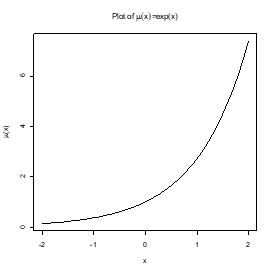
\includegraphics[width=0.5\linewidth]{figs_L14/f1} \end{center}
\end{frame}

\begin{frame}{}
\protect\hypertarget{section}{}
For the binomial, consider \(\hat p_i=Y_i/n_i\), where
\(Y_i \sim \mathcal {Bin}(n_i,\ p_i)\). Of course \(p\) must be bound
between 0 and 1 and intuitively would be a continuous function of
\(\pmb x_i^r\). In order to maintain these characteristics, one
possibility is to set
\(p_i=\frac {e^{\pmb x_i^r \pmb \beta}} {1+e^{\pmb x_i^r \pmb \beta} }.\)

This corresponds to the logit link. (Can you show?) The function above
is plotted to the right, for one continuous covariate, for
\(\beta_0 = 0\) and \(\beta_1=1\); this demonstrates the signature
`slanted S' shape. However, for certain applications, this may not be
apparent since the range of \(x\) values may only cover a portion of the
`S'.

\begin{center}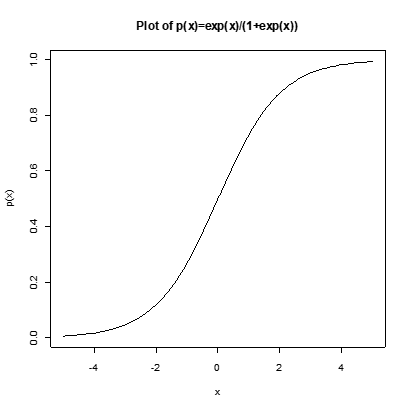
\includegraphics[width=0.5\linewidth]{figs_L14/f2} \end{center}
\end{frame}

\begin{frame}{Interpreting effects for loglinear and logistic models}
\protect\hypertarget{interpreting-effects-for-loglinear-and-logistic-models}{}
There are two common situations where loglinear models are used:

\begin{enumerate}
[(i)]
\tightlist
\item
  when the outcome variable is log transformed to be approximately
  normal
\item
  when a log link is used for a count variable (e.g., Poisson
  regression).
\end{enumerate}

For such models, we can easily derive multiplicative effects. Let's
first consider case (i); for simplicity, consider the simple model
\(ln(Y_{ij})= \beta_0+ \beta_1 x_{ij} + \epsilon_{ij}\), for subject
\(i\) and time \(j\).

Then, \(Y_{ij} = e^{\beta_0+ \beta_1 x_{ij} + \epsilon_{ij}}\), which
implies that
\(E(Y_{ij} |X_{ij} =x_{ij} )= E[e^{\beta_0+ \beta_1 x_{ij} + \epsilon_{ij}}] =E[e^{\beta_0+ \epsilon_{ij} } e^{\beta_1 x_{ij}}] =e^{\beta_1 x_{ij} } E[e^{\beta_0+ \epsilon_{ij}}] =e^{ \beta_1 x_{ij} } c\)

and \(E[Y_{ij}| X_{ij}] = x_{ij} +1]=e^{\beta_1 (x_{ij} +1)} c\), where
\(c\) is a constant. From these, \(E[Y|x+1]/E[Y|x]=e^{\beta_1 }\). In
words, the multiplicative increase in the mean of \(Y\) for a 1-unit
increase in \(x\) is \(e^{\beta_1 }\). Or the relative increase in the
mean of \(Y\) for a 1-unit increase in \(x\) is
\(100(e^{\beta_1 }-1)\%\).
\end{frame}

\begin{frame}{}
\protect\hypertarget{section-1}{}
Case (ii) (log link in generalized linear models) differs from (i) in
that the natural log is taken on \(E[Y]\) and not \(Y\) itself. Consider
(1), with one simple linear predictor:
\(ln(\mu_i)= \beta_0+ \beta_1 x_i\)

Exponentiating both sides yields \(\mu_i=e^{\beta_0+ \beta_1 x_i }\)

Thus, \(\beta_1\) also has a multiplicative effect interpretation, as
before. The log is the natural link for Poisson outcomes and
consequently beta parameters associated with predictors in Poisson
regression have relative increase interpretations when the natural link
is used.
\end{frame}

\begin{frame}{}
\protect\hypertarget{section-2}{}
Some things differ between cases (i) (logged outcome for a normal theory
model) and (ii) (log link for a count outcome) above.

\begin{itemize}
\item
  In (i) we model the mean of the logged \(Y\) values, so inverting back
  to original units will yield the geometric mean (usually closer to the
  median than the arithmetic mean for right skewed distributions). In
  (ii), we model the log of the mean (where `mean' is the arithmetic
  mean).
\item
  For (i), if we assume that normal theory model assumptions are met
  after log transformation (including constant variance), then equal
  variances on that scale will imply that variances on the original
  scale will increase as the mean of \(Y\) increases. This is why the
  log transformation is sometimes used to `stabilize' variance. In (ii),
  we assume constant variance on the regular scale {[}i.e., for \(Y\),
  not \(log(Y)\){]}
\end{itemize}
\end{frame}

\begin{frame}{}
\protect\hypertarget{section-3}{}
For logit link models, odds ratios are derived readily. To illustrate
this using the simple linear logit model:
\(log[(\pi (x)/(1-\pi (x))]= \beta_0+ \beta_1 x\), where
\(\pi (x)=P(Y=1|X=x)\).

Exponentiating both sides yields
\(\pi (x)/(1-\pi (x))=e^{\beta_0+ \beta_1 x}. \ \ \ \ \ (4)\)

But note that
\(\pi (x+1)/(1-\pi (x+1))=e^{beta_0+ \beta_1 (x+1)} \ \ \ \ \ \ (5)\)

Thus, if we divide (5) by (4), we yield an odds ratio (a ratio of
ratios):
\(\frac {\pi (x+1)/(1-\pi (x+1))} {\pi (x)/(1-\pi (x))} = e^{\beta_1}\).

In words, for a 1-unit increase in \(x\), the odds of an event
(associated with \(Y=1\)) increases \(e^{\beta_1}\) times.
\end{frame}

\hypertarget{augmenting-gzlms-to-account-for-correlated-responses}{%
\section{Augmenting GzLMs to account for correlated
responses}\label{augmenting-gzlms-to-account-for-correlated-responses}}

\begin{frame}{Generalized estimating equations (GEE)}
\protect\hypertarget{generalized-estimating-equations-gee}{}
One option in modeling correlated non-normal outcome data is to use
generalized estimating equations (GEE) that can be applied to GzLMs for
longitudinal data. To begin, initial estimates are obtained assuming
data are independent, using the usual GzLM methodology. GEE are then
applied iteratively to obtain estimates of interest accounting for the
correlated data.

GEE does not work with a true likelihood and thus does not actually fit
a true covariance matrix. Rather, it uses what is called a working
covariance matrix. But the forms of the working structures that can be
used are ones we are familiar with (e.g., AR(1), exchangeable - i.e.,
CS).
\end{frame}

\begin{frame}{}
\protect\hypertarget{section-4}{}
The specific steps for GEE are as follows. This is just a sketch; for
more detail see the SAS Help Documentation or other references listed at
the end of this subsection.

\begin{enumerate}
\tightlist
\item
  Use standard GzLM theory to obtain initial estimates of
  \(\pmb \beta\).
\item
  Compute working correlations based on standardized residuals, the
  current estimate of \$\pmb \beta \$ and the assumed covariance
  structure.
\item
  Compute an estimate of \(\pmb V_i = Var[\pmb Y_i]\).
\item
  Update the estimate of \(\pmb \beta\) using the new estimate of
  \(\pmb V_i\).
\item
  Repeat steps 2-4 until convergence.
\end{enumerate}

GEE is considered a general type of quasi-likelihood estimation (QLE)
since it is an estimation method that is not built on maximum likelihood
principles and only requires the form of the mean, the variance as a
function of the mean, correlation parameters (via the `working'
correlation matrix), and scale parameter (see Liang and Zeger, 1986).
\end{frame}

\begin{frame}{}
\protect\hypertarget{section-5}{}
After the GEE process is complete, model-based and empirical forms of
\(Var[\pmb {\hat \beta}]\) can be obtained in order to conduct tests
involving \(\pmb \beta\). The forms of these variances (e.g.,
\textbf{see Hedeker, p.~137-38}) are analogous to the model-based and
empirical forms of variances of beta estimates in mixed models.

The default in SAS is to use the empirical estimates (sometimes also
called robust, or sandwich estimators). These estimators have the
advantage that they are robust to miss-specifications of the (working)
covariance structure.

However, for smaller sample sizes the use of residuals often leads to an
underestimated standard error; the smaller the sample size, the worse
the underestimation. (Yu Zhang, examined this issue for count outcomes
and successfully defended his Master's Thesis on this topic.)
\end{frame}

\begin{frame}{}
\protect\hypertarget{section-6}{}
In order to obtain the model-based variance estimators, include MODELSE
as an option in the REPEATED statement. If this is done, there are
various ways to adjust the variance estimates by scale parameter
estimates, some of which are listed below (in SAS).

\begin{itemize}
\item
  Adjust the variance estimates by a scale parameter by including
  \(\phi\) as a scalar in \(Var[\pmb Y_i]\) within the GEE estimation
  process. This can be achieved by not including a SCALE or NOSCALE
  option in the MODEL statement. A standardized Pearson statistic is
  used to estimate \(\phi\).
\item
  Fix the scale parameter at 1 in the GEE estimation process but then
  adjust variance estimates by a factor of \(\sqrt \phi\), using a
  Pearson or deviance statistic to estimate \(\phi\). In the MODEL
  statement, include the PSCALE option to use the Pearson statistic or
  the DSCALE option to use the deviance statistic.
\item
  Do not adjust variance estimates by a scale parameter. This can be
  achieved by including the NOSCALE option in the MODEL statement.
\end{itemize}
\end{frame}

\begin{frame}{}
\protect\hypertarget{section-7}{}
Note that for GzLM fits, the inclusion of the scale parameter in the GEE
process {[}a scalar in the equation of \(Var[Y_i]\){]} will affect
\(Var[\pmb {\hat \beta}]\), but not \(\pmb {\hat \beta}\) itself, as is
the case for standard GzLMs.

For GzLMs, the theory is developed for independent responses from
subjects (i.e., cross-sectional data). GEE is then an extension for
clustered data (e.g., longitudinal data). Thus, the notation of GzLMs
can be modified to account for this. Specifically, we can use
\(\eta _{ij} =\pmb x_{ij} ^r \pmb \beta\) to denote linear predictor for
subject \(i\) at time \(j\); \(\pmb x_{ij} ^r\) is a row vector with
elements \(x_{vij}\), where \(v\) denotes the covariable (formerly
denoted by \(j\); \(j\) is now used to index time). The response for
subject \(i\) at time \(j\) is then denoted as \(Y_ij\). Other
quantities can be generalized similarly (e.g., \textbf{see Hedeker,
2006}).
\end{frame}

\hypertarget{references}{%
\section{References}\label{references}}

\begin{frame}{References:}
\protect\hypertarget{references-1}{}
Liang K-YL, Zeger S. (1986) Longitudinal Data Analysis Using Generalized
Linear Models, Biometrika 73(1): 13-22. {[}Original article on GEE.{]}

Hedeker D., Gibbons RD. (2006) Longitudinal Data Analysis, Wiley, NJ,
Chapter 8: Generalized Estimating Equations (GEE) Models.

SAS Help Documentation: SAS/STAT, The GENMOD Procedure, Details,
Generalized Estimating Equations, v. 9.1 and 9.2, Cary, NC.
\end{frame}

\hypertarget{application}{%
\section{Application}\label{application}}

\begin{frame}{Application of GEE with a count outcome}
\protect\hypertarget{application-of-gee-with-a-count-outcome}{}
Count outcome variables can often be fit with a Poisson distribution,
perhaps with the addition of a scale parameter, if necessary, if there
is over- or under-dispersion. The following count outcome example is
from my work, illustrating a significant association between daily doser
medication use and air pollution. The data are fit using GzLM/GEE. These
data tend to be underdispersed relative to the Poisson distribution
(i.e., the variance tends to be less than the mean).

Code:

\begin{center}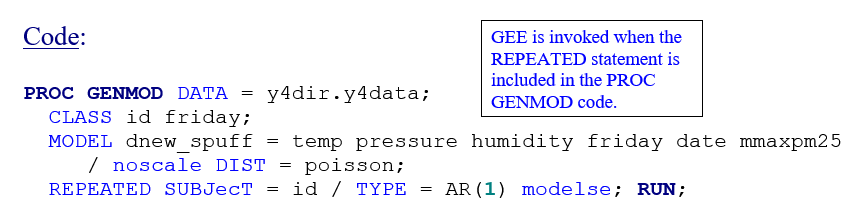
\includegraphics[width=0.6\linewidth]{figs_L14/f3} \end{center}
\end{frame}

\begin{frame}{}
\protect\hypertarget{section-8}{}
Condensed output:

\begin{center}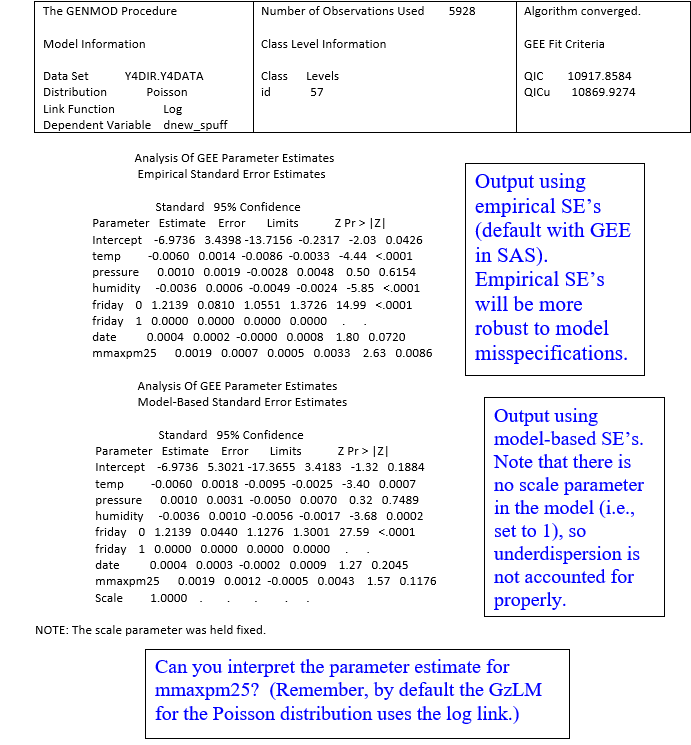
\includegraphics[width=0.8\linewidth]{figs_L14/f4} \end{center}
\end{frame}

\begin{frame}{}
\protect\hypertarget{section-9}{}
If you include the PSCALE or DSCALE options in the MODEL statement, the
model-based SE's will be a bit closer to the SE's using empirical
methods:

Abbreviated output when including PSCALE to the right of `/' in the
MODEL statement:

\begin{center}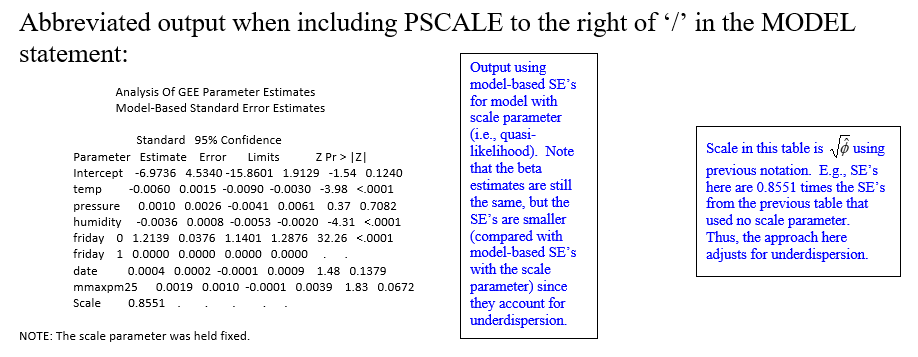
\includegraphics[width=0.8\linewidth]{figs_L14/f5} \end{center}

The `Scale' estimate is \(\sqrt \phi\), and the SE's here are equivalent
to those from the model-based SE's when NOSCALE is used, times
\(\sqrt \phi\). In this case the SE's are still larger than when using
the empirical approach, despite the scale adjustment. When including
DSCALE, the square root of \(\phi\) is 0.8956, so that the adjustment to
the original model-based SE's are even less.
\end{frame}

\begin{frame}{}
\protect\hypertarget{section-10}{}
The following is the partial output obtained when not including any
SCALE or NOSCALE option in the MODEL statement. Here, the phi parameter
is involved in the GEE estimation, but note that the results are not too
different than the previous one in which the variance estimates were
only adjusted after the GEE estimation.

\begin{center}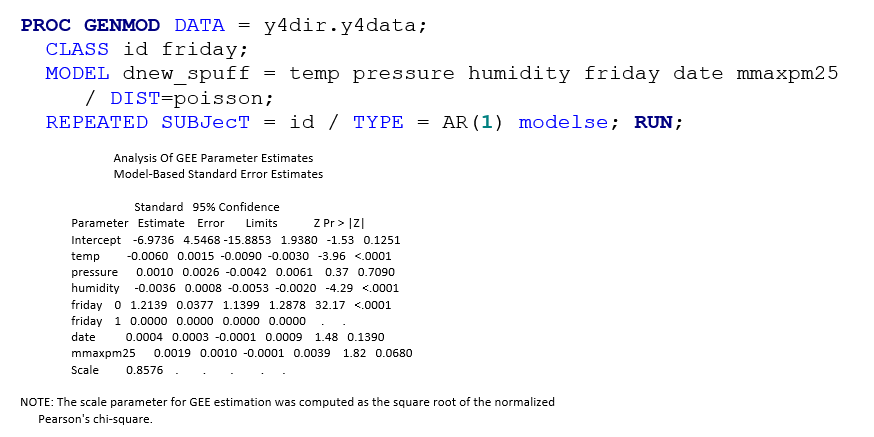
\includegraphics[width=0.8\linewidth]{figs_L14/f6} \end{center}
\end{frame}

\hypertarget{summary}{%
\section{Summary}\label{summary}}

\begin{frame}{Summary}
\protect\hypertarget{summary-1}{}
\end{frame}

\end{document}
